\documentclass{article}
\usepackage[utf8]{inputenc}
\usepackage{graphicx}
\usepackage{caption}
%\documentclass{minimal}
\usepackage{amsmath}
\usepackage{array}

\begin{document}

\title{Medycyna Pola Walki}
\author{Piotr Kwiatkowski}
\date{\today}
\maketitle
\begin{figure}[h]
\centering
    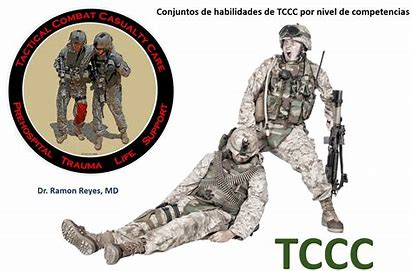
\includegraphics[width=0.5\textwidth]{pictures/zdjecia_Piotr/tccc.jpg}

\end{figure}
\section{Wprowadzenie}
\textbf{Medycyna pola walki} to dziedzina medycyny, która zajmuje się opieką zdrowotną w warunkach konfliktów zbrojnych i sytuacjach kryzysowych.\par Skupia się na szybkim i skutecznym udzielaniu pomocy medycznej rannej osobie w trudnych warunkach, często w terenie, gdzie dostęp do tradycyjnych usług medycznych jest ograniczony.

\section{Zabójcy pola walki}
Najczęstsze przyczyny zgonów na polu walki, których można było uniknąć to:·
\begin{itemize}
    \item około 60\% to krwotoki z kończyn
    \item około 33\% to odma prężna
    \item około 6\% to niedrożność dróg oddechowych
\end{itemize}
\newpage
\section{Protokół MARCH}
\begin{enumerate}
    \item \textbf{M}assive Bleedings
    \item \textbf{A}irways
    \item \textbf{R}espiration
    \item \textbf{C}irculation
    \item \textbf{H}ypothermia, \textbf{h}ypovolemia, \textbf{H}ead injuries
\end{enumerate}


\section{Skala AVPU}

\begin{table}[htbp]
\begin{tabular}{|l|l|}
\hline
ocena          & stan                    \\ \hline
A-alert        & pacjent jest czujny     \\ \hline
V-voice        & pacjent reaguje na głos \\ \hline
P-pain         & pacjent reaguje na ból  \\ \hline
U-unresponsive & pacjent nie reaguje     \\ \hline
\end{tabular}
\end{table}
\section{Matematyka}
\begin{enumerate}
    \item \textbf{Małe twierdzenie Fermata:} Jeśli \( p \) jest liczbą pierwszą, a \( a \) jest liczbą całkowitą taką, że \( a \) nie jest podzielna przez \( p \), to:

\[
a^{p-1} \equiv 1 \pmod{p}
\]
\item \textbf{Twierdzenie Eulera:} Jeśli \( a \) i \( n \) są liczbami całkowitymi, gdzie \( n > 0 \) oraz \( \gcd(a, n) = 1 \), to:

\[
a^{\phi(n)} \equiv 1 \pmod{n}
\]

gdzie \( \phi(n) \) to funkcja Eulera, która zlicza liczby całkowite mniejsze od \( n \) i względnie pierwsze z \( n \).
\end{enumerate}

\end{document}